\documentclass[en]{../../../eplsummary}

\usepackage{multicol}
\usepackage{pgfplots}

\hypertitle{Nonlinear programming}{8}{INMA}{2460}
{Benoît Legat}
{Yurii Nesterov}

\begin{center}
  ``The main fact, which should be known to any person dealing with optimization models,
  is that, in general, \emph{the optimization problems are unsolvable}.''
  \hfill\cite[p.~5]{nesterov1998introductory}
\end{center}

\section{The World of Nonlinear Optimization}
We are interested in the problem
\begin{align*}
  \min & f_0(x)\\
  f_j(x) & \leq 0 & j = 1, \ldots, m\\
  x & \in S.
\end{align*}
where $f_0$ is the \emph{objective} function,
the vector function $f(x) = (f_1(x), \ldots,f_m(x))$ is called the \emph{functional constraint},
the set $S$ is called the \emph{basic feasible set} and the set
\[ Q = \{\, x \in S \mid f_j(x) \leq 0, j = 1, \ldots, m \, \} \]
is called the \emph{feasible set} of the optimization problem.

$S$ stands for \emph{structural} constraints, like non-negativity or boundedness of some variables.
% TODO link that to chapter 4

\begin{itemize}
  \item It is called \emph{unconstrained} if $Q \equiv S \equiv \Rn$ and \emph{constrained} otherwise.
  \item It is called \emph{smooth} if all the $f_i$ are differentiable and \emph{nonsmooth} otherwise.
\end{itemize}

A \emph{method} $\mathcal{M}$ for a \emph{class} $\mathcal{F}$ is given as input a problem $\mathcal{P}$ of $\mathcal{F}$.
Since $\mathcal{M}$ deals with the whole class $\mathcal{F}$,
it does not have the complete description of the problem $\mathcal{P}$ but rather the description of the class $\mathcal{F}$.
In addition it has access to an oracle $\mathcal{O}$ to collect specific information about $\mathcal{P}$.

The pair $(\mathcal{F}, \mathcal{O})$ defines a \emph{model}.
The \emph{peformance} of a method $\mathcal{M}$ on a model $(\mathcal{F}, \mathcal{O})$ is its performance on the \emph{worst} problem $\mathcal{P}_w$ of $\mathcal{F}$ for $\mathcal{M}$.

Once we define what ``a solution $x$ with accuracy $\epsilon$'' means (e.g. $\|x - x^*\| \leq \epsilon$, $|f(x)-f(x^*)| \leq \epsilon$, ...) % TODO do a list
we can define the complexity of the problem $\mathcal{P}$ for the method $\mathcal{M}$
\begin{description}
  \item[Analytical complexity]
    The number of calls to the oracle required for an accuracy $\epsilon$.
  \item[Arithmetical complexity]
    The number of arithmetic operations required for an accuracy $\epsilon$,
    including operations done by the oracle and by the method.
\end{description}

We will analyse three type of oracle of input $x \in \mathbb{R}^n$%TODO on les analyse vraiment tous ?
\begin{description}
  \item[Zero-order oracle] outputs the value $f(x)$.
  \item[First-order oracle] outputs the value $f(x)$ and the gradient $f'(x)$.
  \item[Second-order oracle] outputs the value $f(x)$, the gradient $f'(x)$ and the Hessian $f''(x)$.
\end{description}

\subsection{Global optimization}
The purpose of this section is to show that global optimization is impossible and we should work on smaller classes of problems.

Clearly, if we do not make any continuity assumption on the objective, the oracle won't give us a lot of information.
Also, since we do not consider that $f$ is convex, we cannot search for the \emph{global} optimal solution in an infinite domain.

Let % TODO the objective is f or f_0 ? f is (f_1, ..., f_m)...
\[ Q = B_n = \{\, x \in \Rn \mid 0 \leq x_i \leq 1, i = 1, \ldots, n \,\} \]
and $f_0$ be $L$-Lipschitz continuous
\begin{align*}
  |f(x) - f(y)| & \leq L\|x - y\| & \forall x,y \in B_n.
\end{align*}
We consider here a Zero-order oracle but the lower complexity bound will be the same for a smooth $f_0$ of for higher order oracle~\cite[p.~18]{nesterov1998introductory}.

The grid method $\mathcal{G}(p)$ consists in calling the oracle at all the $(p+1)^n$ points
of the set $\{0,1/p,2/p,\ldots,1\}^n$ and return the point of the grid giving the minimum value for the objective $f_0$.

\begin{tabular}{lll} % TODO find exact bounds
  $L$-Lipschitz with norm & $\mathcal{G}$ & Lower\\
  2
  & $\big(\lfloor \frac{L\sqrt{n}}{2\epsilon} \rfloor + 2\big)^n$
  & $\big(\lfloor \frac{L}{2\epsilon} \rfloor\big)^n$\\
  $\infty$
  & $\big(\lfloor \frac{L}{2\epsilon} \rfloor + 2\big)^n$
  & $\big(\lfloor \frac{L}{2\epsilon} \rfloor\big)^n$
\end{tabular}

\subsection{Nonlinear optimization}
\subsubsection{Function classes}
If $f$ is differentiable at $\bar{x}$ then for $y \in \Rn$ we have
\[ f(x) = f(\bar{x}) + \langle f'(\bar{x}), y-\bar{x}\rangle + o(\|y-\bar{x}\|) \]
where $o(r)$ is some function of $r > 0$ such that $\lim_{r \downarrow 0} \frac{1}{r}o(r) = 0$ and $o(0) = 0$.

\begin{mynota}
  We denote by $C^{k,p}_L(Q)$ the class of functions $f$ that are $k$ times continuously differentiable on $Q$
  and its $p$th derivative is Lipschitz continuous on $Q$ with the constant $L$:
  \[ \| f^{(p)}(x) - f^{(p)}(y) \| \leq L \| x - y \| \]
  for all $x,y \in Q$.
\end{mynota}

We have seen that we cannot win the game of optimization in General or with a Lipschitz continuous fonction.
Any function can be approximated as close as possible with a smooth function so with need First or Second order Lipschitz.
\paragraph{First order Lipschitz}
\begin{mylem}
  A function $f \in C^2$ belongs to $C^{2,1}_L(\Rn) \subseteq C^{1,1}_L(\Rn)$ if and only if
  \[ \| f''(x) \| \leq L \]
  for all $x \in \Rn$.
\end{mylem}

\begin{multicols}{2}
  \begin{myprop}
    Let $f \in C^{1,1}_L$. Then for any $x,y \in \Rn$ we have
    \begin{equation}
      \label{eq:lipschitzfirst}
      | f(y) - f(x) - \langle f'(x), y-x \rangle| \leq \frac{L}{2} \|y - x\|^2.
    \end{equation}
  \end{myprop}

  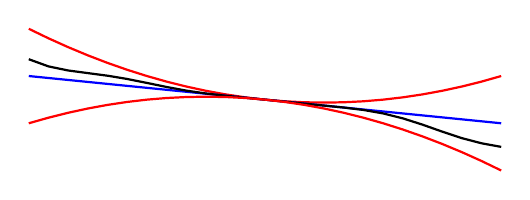
\begin{tikzpicture}[x=3cm,y=0.6cm]
    \draw[color=red, thick, domain=-1:1] plot
    (\x, {-\x/2+(\x)^2});
    \draw[color=blue, thick, domain=-1:1] plot
    (\x, {-\x/2});
    \draw[thick, domain=-1:1] plot
    (\x, {-(\x)^3/2 - \x*\x*sin(60-\x*420)/6-\x/2});
    \draw[color=red, thick, domain=-1:1] plot
    (\x, {-\x/2-(\x)^2});
  \end{tikzpicture}
\end{multicols}

\paragraph{Second order Lipschitz}
We have the exact same property thant for First order Lipschitz with $f'$ since $f'$ is first order Lipschitz
\begin{myprop}
  Let $f \in C^{2,2}_M$. Then for any $x,y \in \Rn$ we have
  \[ | f'(y) - f'(x) - \langle f''(x), y-x \rangle| \leq \frac{M}{2} \|y - x\|^2. \]
\end{myprop}
\begin{mycorr}
  Let $f \in C^{2,2}_M$. Then for any $x,y \in \Rn$ we have
  \begin{equation}
    \label{eq:lipschitzsecondeig}
    f''(x) - MrI_n \leq f''(y) \leq f''(x) + MrI_n.
  \end{equation}
  where $r = \|y-x\|$.
  Remember that $A \leq B$ means that $B-A$ is positive semidefinite.
\end{mycorr}

If $f \in C_M^{2,2}$ and there is a local minimum $x^*$ such that $f'(x^*) = 0$ and $f''(x^*)$ is positive definite.
Let $0 < l \leq L < \infty$ such that the eigenvalues of the hessian $f''(x^*)$ are in the interval $[l,L]$.

Since $f'(x^*)=0$, we can see that $f'(x) = G(x)(x-x^*)$ where
$G(x) = \int_0^1 f''(x^* + \tau(x-x^*)) \dif \tau$.
If we use \eqref{eq:lipschitzsecondeig} and integrate,
we see that the eigenvalues of $G(x)$ are between $l-\frac{r}{2}M$ and $L+\frac{r}{2}M$
where $r = \|x - x^*\|$.

What that means is that from a point $x$,
the directional derivative in the direction of $x^*$ $p = \frac{x^*-x}{\|x^*-x\|}$ which is
$p^T f'(x) = -(x-x^*)^TG(x)(x-x^*)/\|x^*-x\|$ is between $-(L+\frac{r}{2}M) r$ and $-(l-\frac{r}{2}M) r$.
\begin{multicols}{2}
  We see that this direction is always a decrease for $x \in B[x^*, \bar{r}]$ where $\bar{r} \eqdef \frac{2l}{M}$.
  Geometrically, that means that there is no hill between $x$ and the target, the path is monotone to $x^*$.
  Also the decrease is bounded from both sides.
  However, this direction is ideal since we do not know $x^*$.

  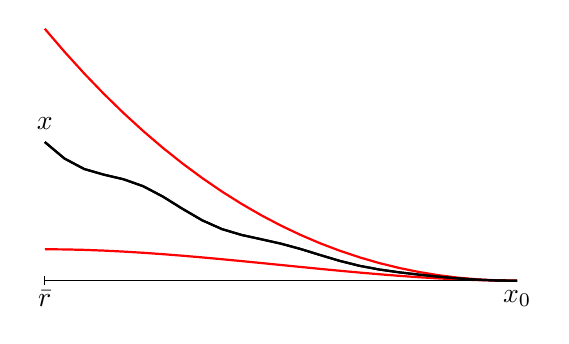
\begin{tikzpicture}[x=3cm,y=0.6cm]
    % derivative should be between xl - 1/2*x^2M and xL + 1/2*x^2M
    % I fix l = 1, L = 2 and M = 1 so bar{r} = 2
    % I want the derivative to be 1.5*x + sin(x) * x^2
    % So the function is 1.5x^2/2 - cos(x) * x^2 + 2sin(x)*x + 2cos(x)
    % Or                 1.5x^2/2 - (k^2*cos(k*x) * x^2 + k*2*sin(k*x)*x + 2cos(k*x)) / k^3
    % I set k to 10 to increase frequency of noise
    \draw[color=red, thick, domain=-2:0] plot
    (\x, {(\x)^2 + abs(\x)^3/6}); % 2/2x^2 + 1/6x^3
    \draw[color=red, thick, domain=-2:0] plot
    (\x, {(\x)^2/2 - abs(\x)^3/6}); % 1/2x^2 + 1/6x^3
    \draw[thick, domain=-2:0] plot
    (\x, {1.5*(\x)^2/2 + (-100*cos(10*180/pi*(\x))*(\x)^2 + 10*2*sin(10*180/pi*(\x))*(\x) + 2*cos(10*180/pi*(\x))-2)/2/1000}); % 1/2x^2 + 1/6x^3
    \draw[thick, domain=-2:0] plot
    (\x, {1.5*(\x)^2/2 + (-100*cos(10*180/pi*(\x))*(\x)^2 + 10*2*sin(10*180/pi*(\x))*(\x) + 2*cos(10*180/pi*(\x))-2)/2/1000}); % 1/2x^2 + 1/6x^3
    \node[above] at (-2, 3) {$x$};
    \node[below] at (0, 0) {$x_0$};
    \draw (-2, 0) -- (0,0);
    \draw (-2, 0.1) -- (-2,-0.1);
    \node[below] at (-2, 0) {$\bar{r}$};
  \end{tikzpicture}
\end{multicols}


\subsection{Local methods in unconstrained minimization}
\begin{mydef}
  We call a sequence $\{a_k\}_{k=1}^\infty$ a \emph{relaxation sequence} if $a_{k+1} \leq a_k$ for all $k \geq 0$.
\end{mydef}
Remember that every non-increasing sequence bounded from below is Cauchy.
If we generate a relaxation sequence $\{f(x_k)\}_{k=0}^\infty$ and $f$ is bounded from below it converges.

\subsubsection{Gradient method}
The gradient method iteration is
\begin{equation}
  \label{eq:graditer}
  x_{k+1} = x_k - h_kf'(x_k).
\end{equation}
If follows the steepest descent $f'(x_k)$.
$h_k$ can be fixed a priori to constant or a function of $k$, e.g. $h/\sqrt{k+1}$ for some constant $h$.
But it can also be computed at each iteration.
Theoritically, we would like to pick
\[ h_k = \argmin_{h \geq 0} f(x_k - hf'(x_k)). \]
That is called a \emph{full relaxation}.

In practice we rather use the Goldstein-Armijo rule
\[ \alpha\langle f'(x_k), x_k - x_{k+1}\rangle \leq f(x_k) - f(x_{k+1}) \leq \beta\langle f'(x_k), x_k - x_{k+1}\rangle \]
\begin{multicols}{2}
  \noindent
  which in the case of the gradient method \eqref{eq:graditer} is
  \[ \alpha h_k\|f'(x_k)\|^2 \leq f(x_k) - f(x_{k+1}) \leq \beta h_k\|f'(x_k)\|^2 \]
  since $x_k - x_{k+1} = -h_kf'(x_k)$.

  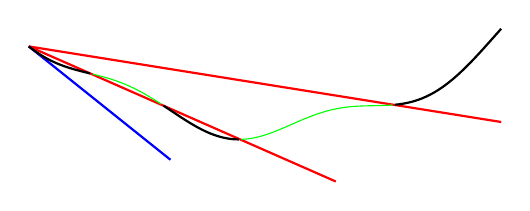
\begin{tikzpicture}[x=3cm,y=0.6cm]
    \draw[color=red, thick, domain=0:2] plot
    (\x, {-0.2*4*\x+1.75});
    \draw[color=red, thick, domain=0:1.3] plot
    (\x, {-0.55*4*\x+1.75});
    \draw[color=blue, thick, domain=0:0.6] plot
    (\x, {-4*\x+1.75});
    \draw[thick, domain=0:0.26] plot
    (\x, {2*(\x-1)^2 - cos(\x*420)/4});
    \draw[green, domain=0.27:0.56] plot
    (\x, {2*(\x-1)^2 - cos(\x*420)/4});
    \draw[thick, domain=0.57:0.89] plot
    (\x, {2*(\x-1)^2 - cos(\x*420)/4});
    \draw[green, domain=0.90:1.54] plot
    (\x, {2*(\x-1)^2 - cos(\x*420)/4});
    \draw[thick, domain=1.55:2] plot
    (\x, {2*(\x-1)^2 - cos(\x*420)/4});
  \end{tikzpicture}
\end{multicols}

\paragraph{First order Lipschitz}
If $f \in C^{1,1}_L$, \eqref{eq:lipschitzfirst} with \eqref{eq:graditer} becomes
\[ f(x_{k+1}) \leq f(x_k) - h_k\Big(1 - \frac{h_k}{2}L\Big) \|f'(x_k)\|^2. \]

We see that for $0 \leq h_k \leq 2/L$, $\{f(x_k)\}_{k=0}^\infty$ is a relaxation sequence.
We decrease at least as much as
\[ f(x_{k+1}) \leq f(x_k) - \frac{w}{L} \|f'(x_k)\|^2 \]
where $w = 1/2$ for a constant $h_k = 1/L$ or for a full relaxation and $w = 2\alpha(1-\beta)$ for Goldstein-Armijo.

Summing for $k = 0, \ldots, N-1$ we get
\[ \frac{w}{L} \sum_{k=0}^N \| f'(x_k) \|^2 \leq f(x_0) - f(x_N) \leq f(x_0) - f^*. \]
If we define $g_N^* = \min_{0 \leq k \leq N} g_k$ we have
\[ g_N^* \leq \frac{1}{\sqrt{N+1}} \Big[ \frac{L}{w} (f(x_0) - f^*) \Big]^2. \]

Note that we cannot say anything about the rate of convergence of the sequence $\{f(x_k)\}$ or $\{x_k\}$
and without additional very strict assumption we cannot guarantee the convergence to a minimum.
The fact that $\|f(x_k)\| \to 0$ as $k \to \infty$ only ensures us that we converge to a stationary point.
%TODO lower bound are not known + cite

\paragraph{Second order Lipschitz}
If $f \in C^{2,2}$ and there is a local minimum $x^*$ such that $f'(x^*) = 0$ and $f''(x^*)$ positive definite.
Let $0 < l \leq L < \infty$ such that the eigenvalues of the hessian $f''(x^*)$ are in the interval $[l,L]$. % TODO Same assumption than for Newton, stop restating it

Using $f'(x_k) = G_k(x_k-x^*)$, \eqref{eq:graditer} gives
\[ r_{k+1} = (I-h_kG_k)r_k \]
and we have seen that the eigenvalues of $I-h_kG_k$
are between $1 - h_k(L+\frac{r_k}{2}M)$ and $1 - h_k(l-\frac{r_k}{2}M)$.

If $x_0$ is close enough to a local minimum $x^*$, i.e. $r_0 < \bar{r}$ where $r_k = \|x_k - x_0\|$,
and for all our steps we choose $h_k$ such that $0 \leq h_k \leq \frac{2}{L+\frac{r_k}{2}M}$ then
for $k > 0$, $x_k$ is also be in the ball $B(x^*,\bar{r})$ and
$\{r_k\}$ is a relaxation sequence.

With the step size $h_k = 2/(L+l)$ we can ensure a linear rate of convergence~[Theorem~1.2.4]\cite{nesterov1998introductory}
\[ \|x_k - x^*\| \leq \frac{\bar{r}r_0}{\bar{r}-r_0} \Big(1 - \frac{l}{L+l}\Big)^k. \]
This rate of convergence is called \emph{linear}.

\subsubsection{Newton method}
Initially, the Newton method was proposed for finding a root of a function of one variable $\phi(t)$, $t \in \R$, $\phi(t^*) = 0$.
Using a linear approximation $\phi(t+\Delta t) \approx \phi(t) + \phi'(t)\Delta t$ which gives $t_{k+1} = t_k - \phi(t_k)/\phi'(t_k)$.
It can be generalized for a function $F : \Rn \to \Rn$ where the scheme becomes $x_{k+1} = x_k - [F'(x_k)]^{-1}F(x_k)$.

In \emph{unconstrained} minimization, it is necessary that $f'(x) = 0$ for $x$ to be a local minimum%
\footnote{In constrainted minimization we need to use KKT condition instead}.
Since $f' : \Rn \to \Rn$, we can apply
\begin{equation}
  \label{eq:newton}
  x_{k+1} = x_k - [f''(x_k)]^{-1}f'(x_k).
\end{equation}

This method has two drawbacks.
First, it can break down if $f''(x_k)$ is degenerate.
Second, the Newton process can diverge (see \cite[Example~1.2.4]{nesterov1998introductory}).
To escape from the possible divergence, we can apply a \emph{damped Newton method}
\[ x_{k+1} = x_k - h_k[f''(x_k)]^{-1}f'(x_k) \]
where $h_k > 0$ is the step-size parameter.
At the initial stage when we are far from $x^*$ we can use the same step size strategies than for the gradient method.
At the final stage it is reasonable to choose $h_k = 1$.

From \eqref{eq:newton}, we have
\[ x_{k+1} - x^* = [f''(x_k)]^{-1}[f''(x_k)](x_k - x^*) - [f''(x_k)]^{-1}f'(x_k) \]
so
\[ x_{k+1} - x^* = [f''(x_k)]^{-1}[f''(x_k)-G_k](x_k - x^*). \]
Let $G'_k = f''(x_k)-G_k$, we can see~\cite[p.~36]{nesterov1998introductory} that $\|G'_k\| \leq \frac{r_k}{2}M$.

\paragraph{Second order Lipschitz}
If $f \in C_M^{2,2}(\Rn)$ and there exists a local minimum of $f$ $x^*$ with positive definite Hessian and let $l>0$ be a lower bound for the eigenvalues of $f''(x^*)$.
From \eqref{eq:lipschitzsecondeig}, we know that the eigenvalues of $f''(x_k)$ are greater than $l-Mr_k$.
If $r_k < l/M = \bar{r}/2$, $f''(x_k)$ is positive definite and the eigenvalues of $f''(x_k)$ are smaller than $(l-Mr_k)^{-1}$ so $\|[f''(x_k)]^{-1}\| \leq (l-Mr_k)^{-1}$.
We have
\[ r_{k+1} \leq \frac{Mr_k^2}{2(l-Mr_k)}. \]
One can verify from this equation that if $r_k < 2l/(3M) = \bar{r}/3$, $\{r_k\}$ is a relaxation sequence.
The rate of convergence of this type is called \emph{quadratic}.

\subsubsection{Variable metric method (or quasi-Newton)}
Note that the gradient $f'(x)$ of a nonlinear function $f(x)$ is defined with
respect to the standard Euclidean inner product $\langle x, y\rangle = y^Tx$ on $\Rn$.
If we define $f'_A = A^{-1}f'(x)$ as the gradient and Hessian with respect to $\langle Ax, y\rangle = y^TAx$,
we have the linear approximation
\begin{align*}
  f(y) & = f(x) + \langle f'(x), y-x \rangle + o(\|y-x\|)\\
       & = f(x) + \langle A^{-1}f'(x), y-x \rangle_A + o(\|y-x\|)\\
       & = f(x) + \langle f'_A(x), y-x \rangle_A + o(\|y-x\|)
\end{align*}
The direction $A^{-1}$ is therefore simply the gradient with respect to a different norm.

The scheme can be seen as a gradient method with $h=1$ but with a different norm.

One other way to see the scheme is the minimization at each step of a the quadratic approximation
\begin{align*}
  f(y) & \approx \phi(x) = f(x) + \langle f'(x), y-x \rangle + \langle A(y-x), y-x \rangle
\end{align*}
The minimization gives the step $A^{-1}f'(x)$.
With $A = f''(x)$ we have the classical approximation corresponding to the second order Taylor expansion and the scheme is the Newton method.

\begin{multicols}{2}
  With $A = I/h$ and $0 < h \leq 1/L$, we see with \eqref{eq:lipschitzfirst} that $\phi$ is an upper approximation of $f(y)$.
  The minimum of $\phi$ has a lower value of $\phi$ than $x$, since it is an upper approximation, it is even lower.
  Therefore, we are sure to have a relaxation sequence.

  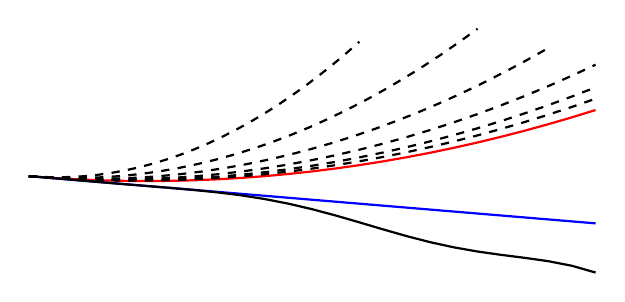
\begin{tikzpicture}[x=6cm]
    \draw[color=red, thick, domain=0:1.2] plot
    (\x, {-\x/2+(\x)^2});
    \draw[color=blue, thick, domain=0:1.2] plot
    (\x, {-\x/2});
    \draw[thick, domain=0:1.2] plot
    (\x, {-(\x)^3/2 - \x*\x*sin(60-\x*420)/6-\x/2});
    \draw[dashed, thick, domain=0:0.7] plot
    (\x, {-\x/2+4.2*(\x)^2});
    \draw[dashed, thick, domain=0:0.95] plot
    (\x, {-\x/2+2.6*(\x)^2});
    \draw[dashed, thick, domain=0:1.1] plot
    (\x, {-\x/2+1.8*(\x)^2});
    \draw[dashed, thick, domain=0:1.2] plot
    (\x, {-\x/2+1.4*(\x)^2});
    \draw[dashed, thick, domain=0:1.2] plot
    (\x, {-\x/2+1.2*(\x)^2});
    \draw[dashed, thick, domain=0:1.2] plot
    (\x, {-\x/2+1.1*(\x)^2});
  \end{tikzpicture}
\end{multicols}
This is the Gradient method.
Actually as we have seen we are also sure to have a relaxation sequence if $\frac{1}{L} < h < \frac{2}{L}$ but it is no more an upper approximation.


\section{Smooth Convex Programming}
\section{Nonsmooth Convex Programming}
\section{Structural Programming}
%In Structural programming, we do not consider constraints as black blox.
%We use the specificity in their structure to remplace them by barriers in the objective.
%The remaining objective is solved using the Newton['s]? scheme.

\biblio
\end{document}
